\documentclass[a4paper]{article}

\usepackage[top=3cm, bottom=2cm, left=2cm, right=2cm]{geometry}
\usepackage{graphicx}
\usepackage{fancyhdr}
\usepackage{scrextend}
\usepackage[hidelinks]{hyperref}
\usepackage{textcomp}
\usepackage{tipa}
\usepackage{caption}
\usepackage{subcaption}
\usepackage{xcolor}

\graphicspath{ {./images/} }

\title{Homework 2 - Machine Learning: Weather Classification}
\author{Edoardo Piroli - 1711234}

\pagestyle{myheadings}
\pagestyle{fancy}
\fancyhf{}

\renewcommand{\headrulewidth}{0pt}
\renewcommand{\footrulewidth}{1pt}

\fancyfoot[C]{Report HW2 - Machine Learning}
\fancyfoot[R]{\thepage}

\begin{document}

\maketitle
\thispagestyle{empty}

\newpage
\tableofcontents
\thispagestyle{empty}
\newpage

\pagenumbering{arabic}

\section{Introduction}
\subsection{Assignment}
The assignment of the homework was to build an image classifier capable of assigning pictures to one of the following classes: \{\textit{RAINY}, \textit{HAZE}, \textit{SUNNY}, \textit{SNOWY}\}; based on how the weather was like at the moment of the picture's capture. In particular, the request was to address the former problem in 2 different ways: 
\begin{enumerate}
\item Defining and training a CNN from scratch for this particular task;
\item Applying transfer learning and fine-tuning on a pre-trained model.
\end{enumerate}
\subsection{Dataset}
The provided datasets\footnote{available here: \href{https://drive.google.com/drive/folders/1UzH28Q8xki8_DMYdDgHxi40-CJ800Kaq}{https://drive.google.com/drive/folders/1UzH28Q8xki8\textunderscore DMYdDgHxi40-CJ800Kaq}} are separated in several different archives and folders. I have chosen to use \textit{MWI-Dataset-1.1\textunderscore 2000} for training, \textit{MWI-Dataset-1.2.4} for testing and \textit{MWI-Dataset-1.2.5} for validation. All these datasets are perfectly balanced, in particular the training dataset is composed by 2000 pictures, 500 per class, while the validation and testing datasets are composed by 400 pictures each, 100 per class. 
\paragraph{Chosen resolution}
The pictures in the datasets don't share a common resolution, this is why I had to resize them in order to be able to train and test. 

In particular, I have chosen to use 299x299 as the pictures' resolution; I have tried other resolutions but this seemed to outperform the others(as expected since the chosen pre-trained model was originally trained on that resolution). I have tried 2 different approaches to resize the pictures:
\begin{enumerate}
\item \textbf{Padded}: Preserving the original aspect ratio, I have resized the longest side to 299, keeping constant the aspect ratio; i.e. proportionately resizing also the other side; and pasted the so-obtained picture on a black 299x299 square; basically adding some padding to the edges. As an example of this resizing process here is one sample picture:

\begin{figure} [h!]
\centering
\begin{subfigure}{0.5\textwidth}
  \centering
  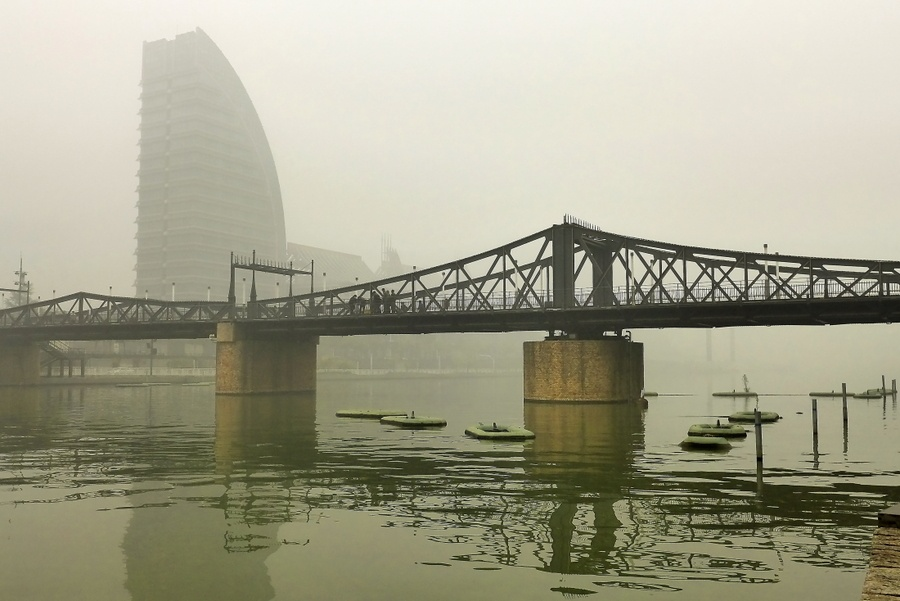
\includegraphics[width=0.99\textwidth]{HAZE-1-1-1_001_ORI.jpg}
  \caption{Original picture with resolution 900x601}
  \label{fig:sub1}
\end{subfigure}%
\begin{subfigure}{0.5\textwidth}
  \centering
  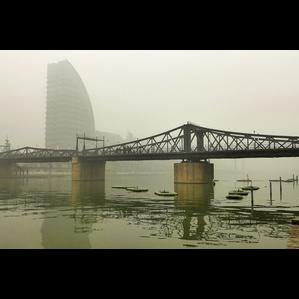
\includegraphics[width=0.99\textwidth]{HAZE-1-1-1_001_ORI_resized.jpg}
  \caption{Resized picture with resolution 299x299}
  \label{fig:sub2}
\end{subfigure}
\label{fig:test}
\end{figure}

\item \textbf{Non-Padded}: I've used the keras.preprocessing.image.ImageDataGenerator flow\textunderscore from\textunderscore directory method to resize the pictures.
\end{enumerate}

Although, differently from what I expected, the second, more classical, method of resizing performed better.
\section{Models}
\subsection{Pre-trained Model}
After looking at the pre-trained models available \href{https://keras.io/applications}{\textcolor{blue}{\underline{here}}}, I have chosen to use the Xception model, characterised by a good ratio between size and accuracy.

The first pre-trained model that I tried is the following one, note that the xception model is completely frozen, i.e. its layers are not going to be modified during the backtracking phase: 
\begin{figure} [h!]
\centering
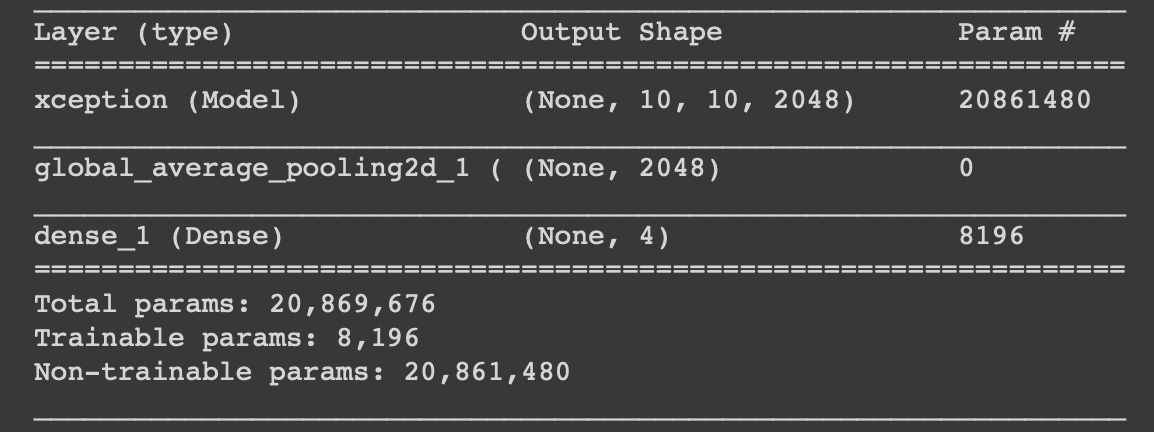
\includegraphics[width=\textwidth]{first_model.png}
\label{fig: first_model}
\end{figure}

Although, also, due to the small number of samples in the training dataset, this model performed poorly, clearly overfitting in less than 10 epochs:
\begin{figure} [h!]
\centering
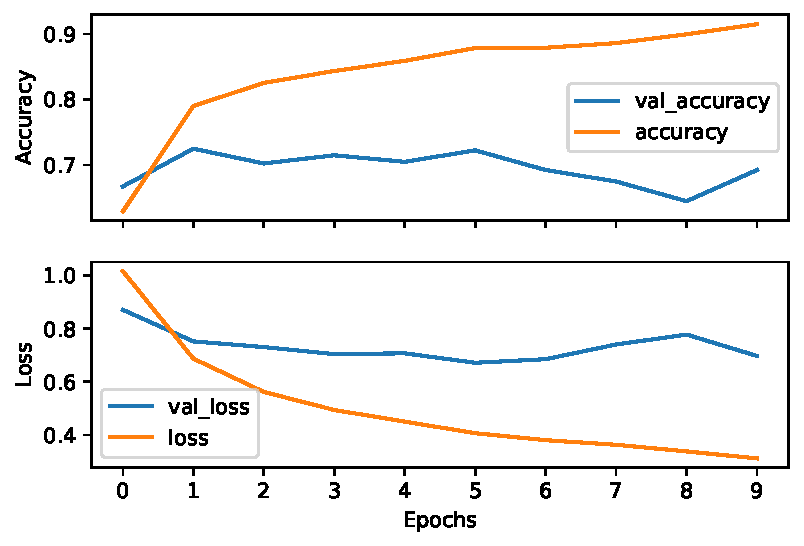
\includegraphics[width=\textwidth]{first_train.pdf}
\label{fig: first_train}
\end{figure}

\newpage
In order to alleviate this problem I have decided to try to add some dropout and regularization terms in the model, the final model which I obtained is the following one:

\begin{figure} [h!]
\centering
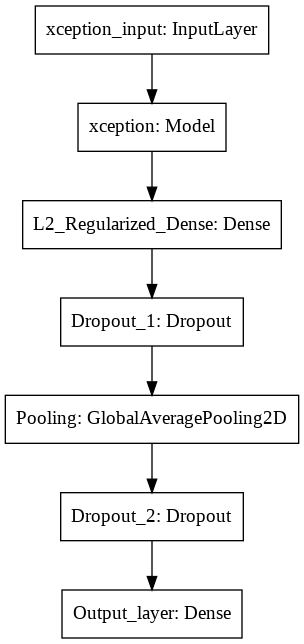
\includegraphics[width=0.5\textwidth]{final_model.png}
\label{fig: final_model}
\end{figure}

\subsection{CNN Model}
In order to be able to better estimate the influence of the pre-trained weights on a niche task, like this one, with few training samples I have decided to use the very same model with the xception model's weights randomly initialized.
\newpage
\section{Training}
\subsection{Hyperparameters}
Both the models share the following hyperparameters:
\begin{itemize}
\item \textbf{Dense size}: The size of the regularized dense layer;
\item \textbf{Regularization term}: The value for the kernel regularizer and the bias one;
\item \textbf{Dropout rate}: Shared among the 2 dropout layers;
\item \textbf{Activation Functions}: I have used 'softmax' for the output layer and 'relu' for the regularized dense layer;
\item \textbf{Optimization Function}: I have just used RMSProp;
\item \textbf{Learning rate}: The value used by RMSProp;
\item \textbf{Rho}: Other value used by RMSProp which I have set to 0.9, as suggested in the keras documentation;
\item \textbf{Epochs}: The number of epochs to train the models;
\item \textbf{Batch size}: I have used 50.
\end{itemize}

\subsection{GridSearch}
In order to try to optimize as much as possible the 2 models I wanted to tune the hyperparameters performing a GridSearch, which in the end I carried out only partially due to time and computational power limitations.

In particular, I wanted to test the following values:
\begin{itemize}
\item \textbf{Dense size}: \{64, 128\};
\item \textbf{Regularization term}: \{0.001, 0.01\};
\item \textbf{Dropout rate}: \{0.3, 0.5\};
\item \textbf{Learning rate}: \{0.0001, 0.001\};
\item \textbf{Epochs}: I have used early stopping on the validation loss with patience=3
\end{itemize}
\end{document}